% Chapter Template

\chapter{Aplicaciones} % Main chapter title

\label{ChapterX} % Change X to a consecutive number; for referencing this chapter elsewhere, use \ref{ChapterX}

\lhead{Capitulo 4. \emph{Aplicaciones}} % Change X to a consecutive number; this is for the header on each page - perhaps a shortened title

%----------------------------------------------------------------------------------------
%	SECTION 1
%----------------------------------------------------------------------------------------

\section{Auto modelamiento}

Juan Cristobal Zagal junto a Hod Lipson \cite{ZagalL09} exploraron el comportamiento de un robot capaz de entrar en un proceso autoreflexivo. Ellos estudiaron a un robot al cual se le programaron dos controladores, uno primitivo (primitive controller) y uno reflexivo (reflective controller) que puede observar al primero.

\begin{figure}[htbp]
	\centering
		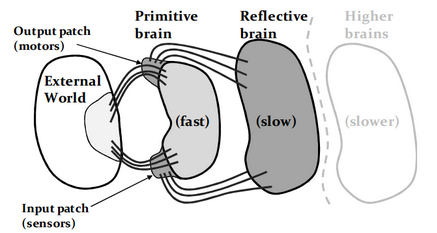
\includegraphics[width=0.7\textwidth]{./Figures/arquitectura_cerebro.png}
		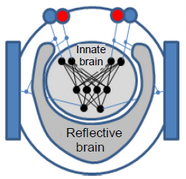
\includegraphics[width=0.4\textwidth]{./Figures/automodelado_epuck.png}
		\rule{35em}{0.5pt}
	\caption[Automodelado]{\textbf{Arriba:} Arquitectura de cerebros anidados usado en el trabajo de J.Zagal y H.Lipson, basado en modelos de M. Minsky. \textbf{Abajo:} Modelo de cerebros implementado en robot e-puck. Ambas imágenes  pertenecen a Juan Cristóbal Zagal.}
	\label{fig:Automodelado}
\end{figure}

El controlador reflexivo es capaz de determinar el control primitivo sin tener acceso directo a sus estados internos, haciendo uso de ingeniería inversa al leer los input/output de éste. Acá se implementa como comportamiento que el robot (e-puck) debe alejarse de luces rojas y acercarse a azules. Se logra con una exploración mínima posible de hardware.

\begin{figure}[htbp]
	\centering
		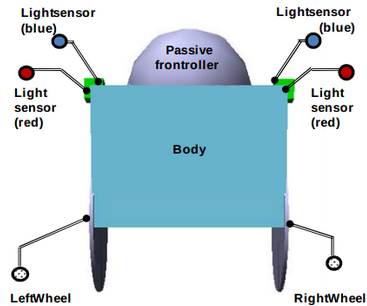
\includegraphics[width=0.4\textwidth]{./Figures/robotTest.png}
		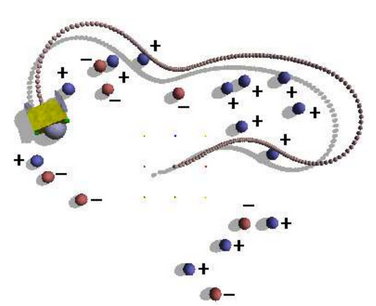
\includegraphics[width=0.5\textwidth]{./Figures/implementacion.png}
		\rule{35em}{0.5pt}
	\caption[Automodelado]{\textbf{Izquierda:} Arquitectura de cerebros anidados usado en el trabajo de J.Zagal y H.Lipson, basado en modelos de M. Minsky. \textbf{Derecha:} Modelo de cerebros implementado en robot e-puck. Ambas imágenes  pertenecen a Juan Cristóbal Zagal.}
	\label{fig:AutomodeladoTest}
\end{figure}


El diagrama del algoritmo que controla todo el proceso que se implementa como comportamiento para recuperarse de fallas puede verse en el anexo.

J. Bongard., V. Zykov y H. Lipson., logran que un robot se recupere de una falla inesperada de forma autónoma. Dicen que el robot puede recuperarse de manera autónoma haciendo uso de su (propio al robot) Self-modeling. Concretamente implementan sus algoritmos en un robot de 4 patas que utiliza una relación entre sus sensores y motores para indirectamente inferir su propia estructura.


Si se remueve una extremidad, el robot es capaz de generar una nueva forma de caminata que le permita cumplir con su misión que es avanzar.
En la figura \ref{fig:AutomodeladoLIPSON}, se describe un esquema del algoritmo. El robot realiza una acción física (A), al azar, luego se ejecuta la mejor acción que se encuentre en (C). A continuación genera varios auto-modelos que coincidan con las lecturas de los sensores obtenidas en (B). Aún no sabe cual es el modelo, por lo que en (C) genera varias acciones posibles que acotan la búsqueda de modelos.Después de varios ciclos de (A) a (C),  el modelo obtenido se utiliza en (E) para generar la secuencia de locomoción. La mejor secuencia de locomoción es probada físicamente en el robot. Se refina el modelo volviendo al paso (B) y en (D) pueden crearse nuevos comportamientos.

\begin{figure}[htbp]
	\centering
		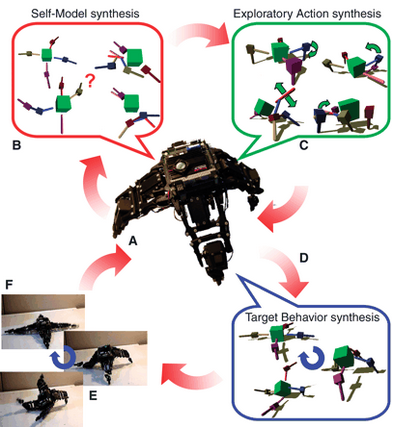
\includegraphics[width=0.5\textwidth]{./Figures/algoritmo_automodelo.png}
		\rule{35em}{0.5pt}
	\caption[AutomodeladoLIPSON]{Esquema del algoritmo que puede usar un robot para desplazarse haciendo uso de Automodelos. Imagen obtenida desde http://creativemachines.cornell.edu}
	\label{fig:AutomodeladoLIPSON}
\end{figure}


\section{Educacion}

%-----------------------------------
%	SUBSECTION 2.1
%-----------------------------------

\subsection{Subsection 2}

%----------------------------------------------------------------------------------------
%	SUBSECTION 3
%----------------------------------------------------------------------------------------
\subsection{Usos Académico}

Un enjambre de robots puede presentar muchas ventajas dentro del aula. Si se tiene un sistema de fácil uso para los alumnos, el profesor puede asignar una tarea a un grupo de estudiantes donde cada uno tiene la responsabilidad de controlar o programar un robot para que el conjunto logre una meta determinada como ordenar unos bloques o hacerse cargo de regar un pequeño huerto. Abusando un poco del concepto de la colectividad, incluso pueden generarse tareas donde cada colegio se especializa en un tipo de tareas para luego juntar los distintos robots y probar cómo interactúan.

Tener un setup con robots que demuestren un comportamiento colectivo puede ser muy ventajoso para ayudar a niños con trastornos como el Asperger a practicar sus habilidades para reconocer estos mismo comportamientos.

\subsection{Usos Militar}

\subsection{Usos Doméstico}
